%!TEX root = ../thesis.tex

\chapter{Isogeometric enhanced SBFEM in 3D}
\section{Introduction}
\paragraph{}
This chapter starts with a mesh generated by the help of the octree based algorithm using STL file directly \citep{Liu2017}.
In this algorithm, the intersection is calculated between the edge of the element and the triangular surface which is an approximation of the exact geometry.
In order to achieve the geometric precision, a point projection method for 3D NURBS surface is presented.
It's computational efficiency is significantly improved by implementing a NURBS surface splitting and by utilizing the strong convex hull property of the NURBS.
The quick hull algorithm is also introduced to construct the convex hull from the control points in 3D.
Alternative method to retain the exact geometry is targeted as well.
The calculation of the intersection in \cite{Liu2017} is replaced by finding that between the edge of the element and the NURBS surface directly.

\paragraph{}
The advantage of the proposed method is that the exact geometry can be retained and hence improves the accuracy of the result.

\paragraph{}
This chapter will be organized as followed:
points projection of the NURBS surface is introduced at the beginning, together with the surface splitting and the convex hull construction.
After that, the calculation of the straight line with the NURBS surface is developed.
Furthermore, a brief introduction on SBFEM formulation in 3D elasticity is presented.
The accuracy and the convergence properties of the proposed method are demonstrated with benchmark problems in the context of linear elasticity.
Some other mesh examples from complex geometric input are also plotted at the end of this chapter.

\section{Projection}
\subsection{Surfaces division}
\label{oct_sc:surface_division}
\paragraph{}
Mapping points back to NURBS surfaces in 3D can be extremely time consuming as there is no known close form mathematical solution.
Every point takes about ten to hundreds iterations before it can find the nearest projection point on the NURBS surface, depending on the size of the projection surface.
However, in the problem that the proposed method is targeting, reasonably complex geometry will be expected.
As a result, points projection back to such kind of NURBS surfaces may takes much more computational time than any others do and it may be necessary to find a more complicated but computational efficient algorithm other than the naive implementation.

\paragraph{}
One concept that can be utilized to improve the efficiency here is the ``divided and conquer''.
As the time complexity of the naive algorithm is $O(n^3)$ where $n$ is directly correlated to the order and the number of control points used to describe the NURBS surfaces, dividing a surface into two generally will make the projection algorithm four times faster than it is before.
Consequently, breaking the origin NURBS surfaces into as many as it can could be a one of the practical practices.

\paragraph{}
Surfaces division can be performed by the help of knot insertion (\ref{lr_sec:nurbs_knot_ins}).
Assuming a NURBS surface defined by two knot vectors\\
$
V_1 = [-1, -1, -1, a_1, a_2, \dots, a_n , 1, 1, 1]
$\\
and
$
V_2 = [-1, -1, -1, b_1, b_2, \dots, b_m, 1, 1, 1]
$.\\
Several knots will be inserted into these two vector so that all interior knots will repeated $p+1$ times and $p$ stands for the order of the NURBS surface in that direction.
After knot insertion, the same NURBS surface will now be described by two new vectors\\
$
V_1^\prime = [-1, -1, -1, a_1, a_1, a_1, a_2, a_2, a_2, \dots, a_n , 1, 1, 1]
$\\
and
$
V_2^\prime = [-1, -1, -1, b_1, b_1, b_1, b_2, b_2, b_2, \dots, b_m, 1, 1, 1]
$.\\
Extraction then can be conducted by take the sub-matrix from the generated control points matrix $P^\prime$ and weight matrix $w^\prime$.

\paragraph{}
Fig.~\ref{oct_fig:nurbs_division} shows a sub-division of breaking a cylinder surface into four smaller ones.

\begin{figure}[h!]
    \centering
    \begin{subfigure}[b]{0.4\linewidth}
        \centering
        \scalebox{0.27}{
            
\includegraphics{octree/images/NURBSParent.png}
        }
        \caption{Original NURBS surface}
    \end{subfigure}
    \begin{subfigure}[b]{0.4\linewidth}
        \centering
        \scalebox{0.25}{
            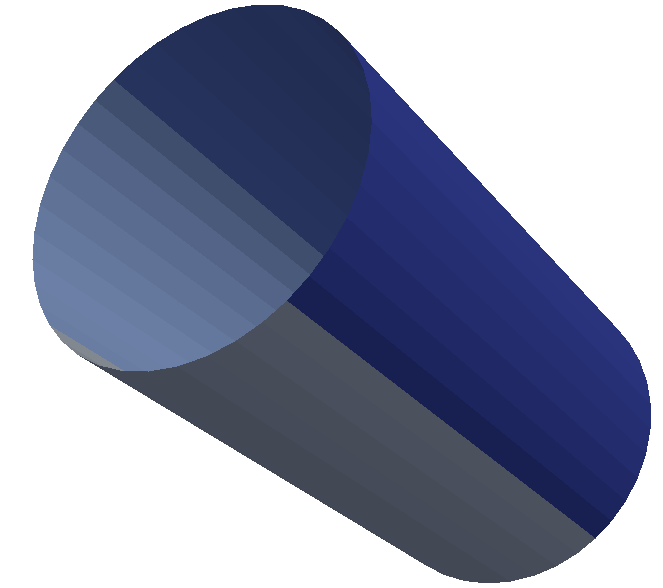
\includegraphics{octree/images/NURBSChildren.png}
        }
        \caption{Subdivided child NURBS surfaces}
    \end{subfigure}
    \caption{NURBS surface subdivision}
    \label{oct_fig:nurbs_division}
\end{figure}

\subsection{Projection algorithm}
\paragraph{}
Point projection algorithm is to find the nearest point in parameter $(u, v)$ on the NURBS surface of the test point.
In the proposed method, all points on the surface is generated based on STL file and are not exactly on the surface.
Some $O(logN)$ algorithms were developed \cite{Edelsbrunner:1985:CED:4007.4011, Chin1983OptimalAF} while presumably large number of tests on polygons is imposed.
Furthermore, the accuracy is out of satisfactory for computer graphics and CAD communities.
As a consequence, a projection algorithm \cite{MA200379} using Newton-Raphson method is introduced to tackle this problem.

\paragraph{}
For a given point $P=(x,y,z)$, its projection on the surface $S(u, v)$ so that the distance $|P-S(u,v)|$ is minimum is targeted.
However, in the proposed method, the existence of the large number of the possible surfaces increase the computational cost significantly.
The projection point for the test point $P$ need to be determined for every existing surface and the one with the smallest minimum distance will be selected.
One possible improvement could be limit the possible surfaces to only a few by utilizing the fact that the NURBS surfaces has been divided into multiple sub-surfaces without interior knot in Sec.~\ref{oct_sc:surface_division}.
Another property that can be utilized is that most of the test point $P$ is expected to be extremely close to its projection on the surface $S(u,v)$.

\paragraph{}
As a consequence, the strong convex hull property can be adopted to limit the number of possible surfaces to less than $2$.
The building of the convex hull is explained in detail in Sec.~\ref{oct_sec:convex_hull}.
The signed distance of the test point to all surfaces' convex hull is calculated and only the surfaces with negative signed distance which indicate that the point is in the convex hull will be selected as candidates.
If no negative distance is detected, a few number (taken as $3$ in the proposed method) of surfaces with minimum signed distance will be selected.

\paragraph{}
In order to find the projection of the test point $P$ on the surface $S$, the vector $r$ is defined as
\begin{equation}
    \mathbf{r} (u, v) =
    \mathbf{S} (u, v) -
    \mathbf{P}
\end{equation}
%
and two scalars $f$ and $g$ are defined as
\begin{equation}
    \left\{
        \begin{array}{rl}
            f (u, v) =
            \mathbf{r}(u, v) \mathbf{\cdot} \mathbf{S}_u (u, v)
            = 0 & \\
            g (u, v) =
            \mathbf{r}(u, v) \mathbf{\cdot} \mathbf{S}_v (u, v)
            = 0 &
        \end{array}
    \right.
\label{oct_eq:projection_function}
\end{equation}
%
In order to solve Eq.~\ref{oct_eq:projection_function}, several notations are introduced
\begin{align*}
    \delta_i &=
        \begin{bmatrix}
            \Delta u \\
            \Delta v
        \end{bmatrix} = 
        \begin{bmatrix}
            u_{i+1} - u_i \\
            v_{i+1} - v_i
        \end{bmatrix} \\
    J_i &=
        \begin{bmatrix}
            f_u & f_v \\
            g_u & g_v
        \end{bmatrix} = 
        \begin{bmatrix}
            \boldmath
            |S_u|^2 + r \cdot S_{uu}        &       S_u \cdot S_v + r \cdot S_{uv} \\
            S_u \cdot S_v + r \cdot S_{uv}  &       |S_v|^2 + r \cdot S_{vv}
        \end{bmatrix} \\
    \kappa_i & = -
        \begin{bmatrix}
            f(u_i, v_i) \\
            g(u_i, v_i)
        \end{bmatrix}
\end{align*}
%
Where all values in matrix $j_i$ can be evaluated at $(u_i, v_i)$.
$2$ by $2$ matrix $\delta_i$ can be determined at step $i$ as
\begin{equation}
    J_i \delta_i = \kappa_i
\end{equation}
%
It can be derived by utilizing $\delta_i$ so that
\begin{subequations}
\begin{align}
    u_{i+1} & = u_i + \Delta u \\
    v_{i+1} & = v_i + \Delta v
\end{align}
\label{oct_eq:projection_iteration}
\end{subequations}
%
The iteration can be concluded as
\paragraph{1}
Is the point coincide with $S(u_i, v_i)$
\begin{equation*}
    |\mathbf{S} (u_i, v_i) - \mathbf{P}| \leq \epsilon_1
\end{equation*}
%
where $\epsilon_1$ stands for the tolerance for distance in Euclidean space.
\paragraph{2}
Is the cosine zero
\begin{align*}
    \frac{
        |\mathbf{S}_u (u_i, v_i) \cdot
        \left(
            \mathbf{S}(u_i, v_i) - \mathbf{P}
        \right)|
    }{
        |\mathbf{S}_u (u_i, v_i)|
        |\mathbf{S}(u_i, v_i) - \mathbf{P}|
    } & \leq \epsilon_2 \\
    \frac{
        |\mathbf{S}_v (u_i, v_i) \cdot
        \left(
            \mathbf{S}(u_i, v_i) - \mathbf{P}
        \right)|
    }{
        |\mathbf{S}_v (u_i, v_i)|
        |\mathbf{S}(u_i, v_i) - \mathbf{P}|
    } & \leq \epsilon_2
\end{align*}
%
where $\epsilon_2$ stands for the tolerance for cosine.
If either of these conditions are met, the iteration is terminated.
Otherwise Eq.~\ref{oct_eq:projection_iteration} is performed to find the parameters $u_{i+1}$ and $v_{i+1}$ for next iteration.
\paragraph{3}
Make sure $u$ and $v$ are within there domains
\begin{align*}
    u_{i+1} & \in [a,b] \\
    v_{i+1} & \in [c,d]
\end{align*}
%
where $a$, $b$, $c$ and $d$ are the lower and upper bounds for the knot vectors of surface $S$.
If the surface is open in $u$ direction
\begin{equation}
    \left\{
        \begin{array}{rl}
            u_{i+1} = a & u_{i+1} < a \\
            u_{i+1} = b & u_{i+1} > b
        \end{array}
    \right.
\end{equation}
%
If the surface is open in $v$ direction
\begin{equation}
    \left\{
        \begin{array}{rl}
            v_{i+1} = c & v_{i+1} < c \\
            v_{i+1} = d & v_{i+1} > d
        \end{array}
    \right.
\end{equation}
%
If the surface is closed in $u$ direction
\begin{equation}
    \left\{
        \begin{array}{rl}
            u_{i+1} = b - ( a - u_{i+1} ) & u_{i+1} < a \\
            u_{i+1} = a + ( u_{i+1} - b ) & u_{i+1} > b
        \end{array}
    \right.
\end{equation}
%
If the surface is closed in $v$ direction
\begin{equation}
    \left\{
        \begin{array}{rl}
            v_{i+1} = d - ( c - v_{i+1} ) & v_{i+1} < c \\
            v_{i+1} = c + ( v_{i+1} - d ) & v_{i+1} > d
        \end{array}
    \right.
\end{equation}
%
\paragraph{4}
The difference between the new parameters $u_{i+1}$ and $v_{i+1}$ and the old ones $u_i$ and $v_i$ is insignificant
\begin{equation*}
    |u(i+1) - u_i| \mathbf{S}_u (u_i, v_i) +
    (v_{i+1} - v_i) \mathbf{S}_v (u_i, v_i) |
    \leq \epsilon_1
\end{equation*}
The iteration will be terminated if this condition is meet.
\subsection{Convex hull in 3D}
\label{oct_sec:convex_hull}
\paragraph{}
The convex hull property of the NURBS surface indicates that all points on the surface must be contained within the convex hull constructed by its control points \citep{SELIMOVIC2009772}
The algorithm in 3D can be very similar to that in 2D as introduced in Sec.~\ref{qdt_sc:convex_hull}.
\begin{enumerate}
    \item Find the most left and right points (points with minimal and maximum $x$) since they are proved to be part of the convex hull.
    \item Connect these two points and use the line to separate other points into two group.
    \item Find the point with maximum distance to the line in step 2 in any group.
    \item Construct a triangle with two points in step 2 and the point in step 3.
    \item Find the point with maximum distance to the triangle in step 4. %5
    \item Construct a tetrahedron with the triangle in step 4 and the point in step 5.
    \item Follow the same procedures in Sec.~\ref{qdt_sc:convex_hull}
\end{enumerate}

\section{Intersection}
\paragraph{}
Instead of projecting all points located on the boundary surfaces to the NURBS surfaces, the exact geometry can be retained by calculating the intersection points directly.
By utilizing the work from Sec.~\ref{oct_sc:surface_division}, the number of the surfaces which may contain the intersection can be limited to a few by \hl{determining} the relationship between their convex hulls and the line.
Only surfaces whose convex hull has intersection with the line will be selected as candidates.
The number of the candidates increase\hl{s} when the mesh becomes coarser as a longer line segment tends to intersect more convex hulls.
On the other hand, when the mesh is refined and the line segment becomes significantly shorter, the number of the candidates decreases at the same time.
A considerable improvement in computational cost can be expected as the time complexity is only meaningful when numerous intersections are calculated.
Only a few intersections need to be determined when the mesh is coarse hence having quite a few candidates at this circumstance may not significantly increase the computational time.
\subsection{Matrix Representation for Rational Bezier Surface} 
\paragraph{}
A tensor-product rational Bézier surface of degree $(p_1,p_2)$ can be expressed as
\begin{equation*}
	\phi(u,v)\in\mathbf{R}^2 \rightarrow \frac{\sum_{i=0}^{p_1}\sum_{j=0}^{p_2}w_{i,j}\mathbf{P}_{i,j}B_i^{p_1}(t)B_j^{p_2}(t) }{\sum_{i=0}^{p_1}\sum_{j=0}^{p_2}w_{i,j}B_i^{p_1}(t)B_j^{p_2}(t)}
\end{equation*}
For the surface, $\mathbf{L}$ and $\mathbf{R}$ with order $(v_1,v_2)$
\begin{equation*}
	\mathbf{L} =
	\begin{bmatrix}
		B_0^{v_1+p_1}(u)B_0^{v_2+p_2}(v) & B_1^{v_1+p_1}(u)B_0^{v_2+p_2}(v) & \dots & B_{v_1+p_1}^{v_1+p_1}(u)B_{v_2+p_2}^{v_2+p_2}(v)
	\end{bmatrix}
\end{equation*}
\begin{equation*}
	\mathbf{R} =
	\begin{bmatrix}
		B_0^{v_1}(u)B_0^{v_2}(v)f_0(u,v) & B_0^{v_1}(u)B_1^{v_2}(v)f_0(u,v) & \dots & B_{v_1}^{v_1}(u)B_{v_2}^{v_2}(v)f_3(u,v)
	\end{bmatrix}
\end{equation*}
Following the same manner in the previous section, it can be derived that 
\begin{equation}
	\mathbf{S}_{\left( (i+k)(v_2+p_2+1)+j+l, l(v1+1)+k\right)} = 
	\frac{\mathbf{C}_k^{v_1}\mathbf{C}_l^{v_2}\mathbf{C}_i^{p_1}\mathbf{C}_j^{p_2}} 
		{\mathbf{C}_{i+k}^{v_1+d_2}\mathbf{C}_{j+l}^{v_2+d_2}}c_{(i,j)}
\end{equation}

\subsection{Property of $\mathbf{M_v}$ Matrix}
As described in the previous sections, the $\mathbf{M_v}$ matrix is defined so that
\begin{equation*}
	\begin{bmatrix}
	\psi_1(t_0) \dots \psi_{m_v}(t_0)
	\end{bmatrix}
	\times
	\mathbf{M_v(\mathbf{P})}
	= \vec{0}
\end{equation*}
where $\mathbf{P}$ is a point on the rational bezier curve/surface.
The order $v$ shall be no less than a critical value and it is proofed to be
\begin{itemize}
	\item $v>max(p-1,1)$ for rational bezier curve
	\item $(v_1,v_2) > (2p_1 -1, p_2 -1)$ or  $(v_1,v_2) > (p_1 -1, 2p_2 -1)$
\end{itemize}
The following properties are proofed in \cite{Laurent2014}
\begin{enumerate}
	\item For all degrees $geq$ critical degree and all point $\in\mathbf{R}^3$ , rank($\mathbf{M_v}(\mathbf{P})$) $<m_v$ if and only if $\mathbf{P}\in$ the closure of $\overline{Im}(\phi)$.
	\item If $\mathbf{P}\in\mathbf{R}^3$ is a point with a unique pre-image by $\phi$, the dimension of the null space of $\mathbf{M_v}(\mathbf{P})^T$ is one. 
	\item $\delta\mathbf{M_v}(\mathbf{P}) = 0$ if $\mathbf{P} \in\overline{Im}(\phi)$
\end{enumerate}
where 
\begin{equation*}
	\delta\mathbf{M_v}(\mathbf{P}) = \prod_{i=1}^{m_v}\sigma_i(\mathbf{M_v}(\mathbf{P}))
\end{equation*}
and $\sigma_i$ is the diagonal of $\Sigma$ in the SVD decomposition of $\mathbf{M_v}(\mathbf{P})=U\Sigma V^T$

\begin{enumerate}
	\setcounter{enumi}{3}
	\item $\forall\mathbf{P}\in\mathbf{R}^3$, $d(\mathbf{P},\overline{Im}(\phi))^{n_1}\leq c_1 \delta\mathbf{M_v}(\mathbf{P})$
	\item $\forall\mathbf{P}\in\mathbf{R}^3$, $\delta\mathbf{M_v}(\mathbf{P})^{n_2}\leq c_2 d(\mathbf{P},\overline{Im}(\phi))^{n_2} $
\end{enumerate}
where $c_1,c_2,n_1,n_2$ are constant.\\
These two properties give a distance function like function of the $M_v$ matrix. When the point get away to the surface, $\delta\mathbf{M_v}$ is getting larger and vice versa.vise visa.
\paragraph{}
If the point is on the curve/surface, in which case $\delta\mathbf{M_v}(\mathbf{P}) = 0$, the corresponding parameter value on the curve/surface can be easily found by a SVD numerically.\\
The computation of the null space of $\mathbf{M_v}(\mathbf{P}) $ will give a single vector $V=[v_1,v_2,\dots,v_{m_v}]$based on 2 and $V$ will be proportional to 
\begin{equation*}
	\begin{bmatrix}
	\psi_1(t_0) \dots \psi_{m_v}(t_0)
	\end{bmatrix}
\end{equation*}
More specifically, it will be proportional to
\begin{equation*}
	\begin{bmatrix}
		B_0^v & B_1^v & \dots
	\end{bmatrix}
\end{equation*}
for the rational bézier curves and
\begin{equation*}
	\begin{bmatrix}
		B_0^{v1}B_0^{v2} & B_0^{v1}B_1^{v2} & \dots
	\end{bmatrix}
\end{equation*}
for the rational bézier surfaces.



\section{Introduction of SBFEM in 3D}
\paragraph{}
A polyhedral cell can be regarded as one of the subdomain\hl{s} in the SBFEM as plotted in Fig.~\ref{oct_fig:sbfem_intro}.
Similar to SBFEM in 2D which has been introduced in Sec.~\ref{iso_section:formulation}, only the boundary surface requires discretization and a scaling center $O$ located at the place where all boundary surfaces of the subdomain are visible is necessary.
%
\begin{figure}
    \centering
    \begin{subfigure}[b]{0.48\linewidth}
        \scalebox{0.5}{
            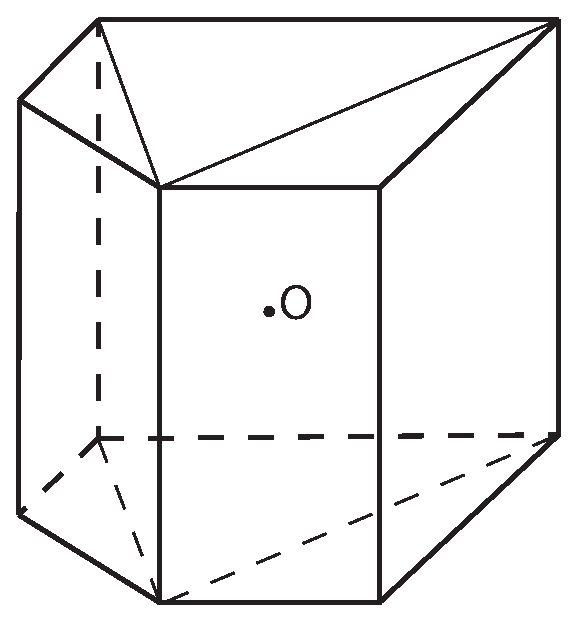
\includegraphics{octree/images/sbfem3d.eps}
        }
        \caption{Scaling center located inside of the subdomain}
        \label{oct_fig:sbfem_intro_a}
    \end{subfigure}
    \begin{subfigure}[b]{0.48\linewidth}
        \scalebox{0.5}{
            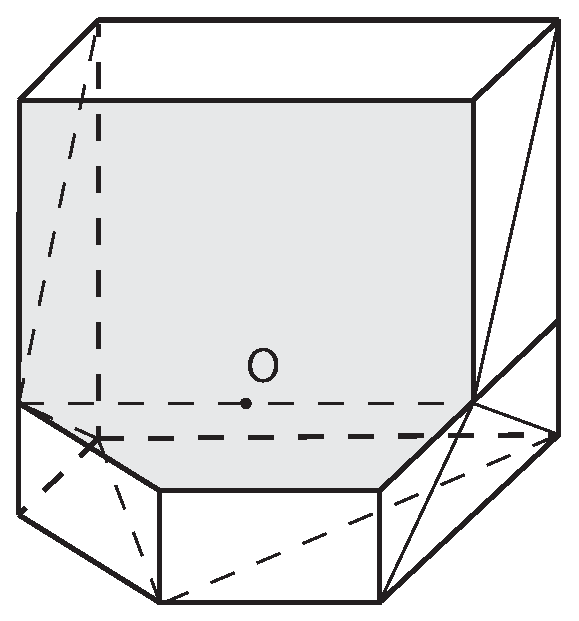
\includegraphics{octree/images/sbfem3d_b.eps}
        }
        \caption{Scaling center located on one of the edges}
        \label{oct_fig:sbfem_intro_b}
    \end{subfigure}
    \caption[Polyhedral SBFEM subdomain in 3D]{Polyhedral subdomain in SBFEM}
    \label{oct_fig:sbfem_intro}
\end{figure}
%
A scaling center on the edge as shown in Fig.~\ref{oct_fig:sbfem_intro_b} is also valid which increases the flexibility and allow\hl{s} the concave subdomain.
In this situation, the triangulated faces containing the scaling center will not be discretized.

\paragraph{}
The transformation between SBFEM coordinate $(\xi, \eta, \zeta)$ and Cartesian coordinate $(x, y, z)$ can be derived from Eq.~\ref{lr_eq:sbfem_boundary_interpolate} and Eq.~\ref{lr_eq:sbfem_scaling} as:
\begin{subequations}
\begin{align}
    x(\xi, \eta, \zeta) & = \xi \hat{x}(\eta, \zeta)  = \xi \mathbf{N}(\eta, \zeta) \mathbf{\hat{x}} \\
    y(\xi, \eta, \zeta) & = \xi \hat{y}(\eta, \zeta)  = \xi \mathbf{N}(\eta, \zeta) \mathbf{\hat{y}} \\
    z(\xi, \eta, \zeta) & = \xi \hat{z}(\eta, \zeta)  = \xi \mathbf{N}(\eta, \zeta) \mathbf{\hat{z}}
\end{align}
\end{subequations}
%
where $(\hat{x}, \hat{y}, \hat{z})$ stands for the point in Cartesian coordinate on the boundary, $(\mathbf{\hat{x}}, \mathbf{\hat{y}}, \mathbf{\hat{z}})$ represents the nodal coordinate vectors and $\mathbf{N}$ is the shape function.
The corresponding Jacobian matrix in 3D on the boundary $(\xi = 1)$ can be expressed as:
\begin{equation}
    \mathbf{J} (\eta, \zeta) =
    \begin{bmatrix}
        x(\eta, \zeta)      &   y(\eta, \zeta)      &   z(\eta, \zeta)  \\
        x(\eta, \zeta),_{\eta}      &   y(\eta, \zeta),_{\eta}      &   z(\eta, \zeta),_{\eta}  \\
        x(\eta, \zeta),_{\zeta}      &   y(\eta, \zeta),_{\zeta}      &   z(\eta, \zeta),_{\zeta}  \\
    \end{bmatrix}
\end{equation}
%
and the displacement interpolation in Eq.~\ref{lr_eq:sbfem_disp_interpolation} becomes
\begin{equation}
    \mathbf{u}(\xi, \eta, \zeta) = \mathbf{N} (\eta, \zeta) \mathbf{u} (\xi)
\end{equation}
%
The linear operator in Eq.~\ref{lr_eq:sbfem_l_operator} becomes
\begin{equation}
    \mathbf{L} = \mathbf{b}_1 (\eta, \zeta) \frac{\partial}{\partial \xi} +
    \frac{1}{\xi}\left(
        \mathbf{b}_2 (\eta, \zeta) \frac{\partial}{\partial \eta} +
        \mathbf{b}_3 (\eta, \zeta) \frac{\partial}{\partial \zeta}
    \right)
\end{equation}
%
Little $b$ matrix in Eq.~\ref{lr_eq:sbfem_little_b} becomes
\begin{subequations}
\begin{align}
    \mathbf{b}_1 (\eta, \zeta) &= \frac{1}{|\mathbf{J}|}
    \begin{bmatrix}
        y,_{\eta} z,_{\zeta} - z,_{\eta} y,_{\zeta} & 0 & 0 \\
        0 & z,_{\eta} x,_{\zeta} - x,_{\eta} z,_{\zeta} & 0 \\
        0 & 0 & x,_{\eta} y,_{\zeta} - y,_{\eta} x,_{\zeta} \\
        0 & x,_{\eta} y,_{\zeta} - y,_{\eta} x,_{\zeta} & z,_{\eta} x,_{\zeta} - x,_{\eta} z,_{\zeta} \\
        x,_{\eta} y,_{\zeta} - y,_{\eta} x,_{\zeta} & 0 & y,_{\eta} z,_{\zeta} - z,_{\eta} y,_{\zeta} \\
        z,_{\eta} x,_{\zeta} - x,_{\eta} z,_{\zeta} & y,_{\eta} z,_{\zeta} - z,_{\eta} y,_{\zeta} & 0
    \end{bmatrix} \\
    \mathbf{b}_2 (\eta, \zeta) &= \frac{1}{|\mathbf{J}|}
    \begin{bmatrix}
        y,_{\zeta} z - z,_{\zeta} y & 0 & 0 \\
        0 & z,_{\zeta} x - x,_{\zeta} z & 0 \\
        0 & 0 & x,_{\zeta} y - y,_{\zeta} x \\
        0 & x,_{\zeta} y - y,_{\zeta} & z,_{\zeta} x - x,_{\zeta} z \\
        x,_{\zeta} y - y,_{\zeta} & 0 & y,_{\zeta} z - z,_{\zeta} y \\
        z,_{\zeta} x - x,_{\zeta} z & y,_{\zeta} z - z,_{\zeta} y & 0
    \end{bmatrix} \\
    \mathbf{b}_3 (\eta, \zeta) &= \frac{1}{|\mathbf{J}|}
    \begin{bmatrix}
        y z,_{\eta} - z y,_{\eta} & 0 & 0 \\
        0 & z x,_{\eta} - x z,_{\eta} & 0 \\
        0 & 0 & x y,_{\eta} - y x,_{\eta} \\
        0 & x y,_{\eta} - y x,_{\eta} & z x,_{\eta} - x z,_{\eta} \\
        x y,_{\eta} - y x,_{\eta} & 0 & y z,_{\eta} - z y,_{\eta} \\
        z x,_{\eta} - x z,_{\eta} & y z,_{\eta} - z y,_{\eta} & 0
    \end{bmatrix}
\end{align}
\end{subequations}
%
Follow the same manner in Sec.~\ref{iso_section:formulation}, the strains can be expressed as
\begin{equation}
    \epsilon(\xi, \eta, \zeta) =
    \mathbf{B}_1 (\eta, \zeta) \mathbf{u} (\xi),_\xi +
    \frac{1}{\xi} \mathbf{B}_2 (\eta, \zeta) \mathbf{u} (\xi)
\end{equation}
%
where
\begin{subequations}
\begin{align}
    \mathbf{B}_1 (\eta, \zeta) & =
    \mathbf{b}_1 (\eta, \zeta) \mathbf{N} (\eta, \zeta) \\
    \mathbf{B}_2 (\eta, \zeta) & =
    \mathbf{b}_2 (\eta, \zeta) \mathbf{N} (\eta, \zeta),_\eta +
    \mathbf{b}_3 (\eta, \zeta) \mathbf{N} (\eta, \zeta),_\xi
\end{align}
\end{subequations}
%
The stress in Eq.~\ref{lr_eq:sbfem_stress} becomes
\begin{equation}
    \sigma(\xi, \eta, \zeta) = \mathbf{D} \left(
        \mathbf{B}_1 (\eta, \zeta) \mathbf{u} (\xi),_\xi +
        \frac{1}{\xi} \mathbf{B}_2 (\eta, \zeta) \mathbf{u} (\xi)
    \right)
\end{equation}
%
and the ODE equation in Eq.~\ref{lr_eq:sbfem_ODE} becomes
\begin{equation}
    \mathbf{E}_0 \xi^2 \mathbf{u}(\xi),_{\xi\xi} +
    (2\mathbf{E}_0 + \mathbf{E}_1^T - \mathbf{E}_1)\xi \mathbf{u}(\xi),_{\xi} -
    (\mathbf{E}_1^T - \mathbf{E}_2) \mathbf{u}(\xi)
    = 0
\label{oct_eq:sbfem_ode}
\end{equation}
%
The coefficient matrices $\mathbf{E}_0$, $\mathbf{E}_1$ and $\mathbf{E}_2$ for element $e$ are expressed as
\begin{subequations}
\begin{align}
    \mathbf{E}_0 = \int_e \mathbf{B}_1^T \mathbf{D} \mathbf{B}_1 |\mathbf{J}| d\eta d\zeta \\
    \mathbf{E}_1 = \int_e \mathbf{B}_2^T \mathbf{D} \mathbf{B}_1 |\mathbf{J}| d\eta d\zeta \\
    \mathbf{E}_2 = \int_e \mathbf{B}_2^T \mathbf{D} \mathbf{B}_2 |\mathbf{J}| d\eta d\zeta 
\end{align}
\end{subequations}
%
The internal nodal forces $\mathbf{q}(\xi)$ on the boundary can be determined as \citep{Son2004a}
\begin{equation}
    \mathbf{q} (\xi) = \xi (
        \mathbf{E}_0 \xi \mathbf{u}(\xi),_\xi +
        \mathbf{E}_1^T \mathbf{u}(\xi)
    )
\label{oct_eq:sbfem_nodal_forces}
\end{equation}
%
$X(\xi)$ is introduced to reduce the order of the ODE in Eq.~\ref{oct_eq:sbfem_ode} as
\begin{equation}
    \mathbf{X} (\xi) =
    \begin{bmatrix}
        \xi^{0.5} \mathbf{u}(\xi) \\
        \xi^{-0.5} \mathbf{q}(\xi)
    \end{bmatrix}
\label{oct_eq:sbfem_x}
\end{equation}
%
substituting Eq.~\ref{oct_eq:sbfem_x} and Eq.~\ref{oct_eq:sbfem_nodal_forces} into Eq.~\ref{oct_eq:sbfem_ode} yields
\begin{equation}
    \xi \mathbf{X} (\xi),_\xi =
    -\mathbf{Z} \mathbf{X} (\xi)
\end{equation}
%
where $Z$ is the hamiltonian matrix
\begin{equation}
    \mathbf{Z} =
    \begin{bmatrix}
        \mathbf{E}_0^{-1} \mathbf{E}_1^T - 0.5 \mathbf{I}   &   -\mathbf{E}^{-1}_0 \\
        -\mathbf{E}_2 + \mathbf{E}_1 \mathbf{E}_0^{-1} \mathbf{E}_1^T   &   -(
            \mathbf{E}_1 \mathbf{E}_0^{-1} - 0.5 \mathbf{I}
        )
    \end{bmatrix}
\label{oct_eq:sbfem_z}
\end{equation}
%
An eigenvalue decomposition of Eq.~\ref{oct_eq:sbfem_z} is performed and it yields
\begin{equation}
    \mathbf{X} (\xi) =
    \begin{bmatrix}
        \Phi_{u1}   &   \Phi_{u2} \\
        \Phi_{q1}   &   \Phi_{q2}
    \end{bmatrix}
    \begin{bmatrix}
        \xi^{-\lambda}  &   0 \\
        0   &   \xi^{\lambda}
    \end{bmatrix}
    \begin{bmatrix}
        \mathbf{c}_1  &   0   \\
        0   &   \mathbf{c}_2
    \end{bmatrix}
\label{oct_eq:sbfem_eigenvalue}
\end{equation}
%
where $\pm\lambda$ is the eigenvalue and $-\lambda$ is corelate to the real parts.
$\Phi$ is part of the matrix of the eigenvector matrix.
$\mathbf{c}_1$ and $\mathbf{c}_2$ stand for the integration constant.
Modal displacements and forces in Eq.~\ref{lr_eq:sbfem_general_sol_str} becomes
\begin{subequations}
\begin{align}
    \mathbf{u}(\xi) &= \mathbf{\Phi}_{u1} \xi^{-\Lambda-0.5\mathbf{I}} \mathbf{c}_1
    \label{oct_eq:sbfem_general_sol_disp} \\
    \mathbf{q}(\xi) &= \mathbf{\Phi}_{q1} \xi^{-\Lambda+0.5\mathbf{I}} \mathbf{c}_2
    \label{oct_eq:sbfem_general_sol_str}
\end{align}
\end{subequations}
%
The stiffness matrix then can be derived as
\begin{equation}
    \mathbf{K} = \Phi_{q1} \Phi_{u1}^{-1}
\end{equation}

\section{Numerical examples}
\section{Pressurized hollow sphere}
\paragraph{}
The problem is a pressurized hollow sphere subjected to internal pressure. The geometry of the problem is described in fig.\ref{oct_fig:ex_pre-hollow-sphere}. 

\begin{figure}[h!]
  \centering
  \scalebox{1}{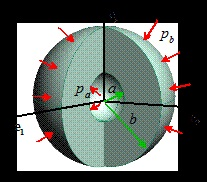
\includegraphics{octree/ex_images/oct_ex_image021.jpg}}
  \caption{Pressurized hollow sphere}
  \label{oct_fig:ex_pre-hollow-sphere}
\end{figure}

\paragraph{}
In the example, the external pressure is set to be zero so that only the internal one is considered. $a=20, b=150, p_a = 10,p_b = 0, E=200,\nu=0.3$. Instead of a quarter of a hollow sphere, a cubic with a spherical hole is analysed. Displacement boundary condition is applied on all of the boundary surface. First order tetrahedral element is adopted to calculated the displacement and stress and compared to the exact solution as in eq.~\ref{oct_eq:ex_hollow_sphere_ana_sol} in spherical coordinate.

\begin{subequations}
\begin{align}
  u & = \frac{1}{2E(b^3-a^3)R^2}\left\{ 2(p_aa^3-p_bb^3)(1-2\nu)R^3+(p_a-p_b)(1+\nu)b^3a^3\right\}\\
  \sigma_{RR} & = \frac{p_aa^3-p_bb^3}{b^3-a^3} - \frac{(p_a-p_b)b^3a^3}{(b^3-a^3)R^3}\\
  \sigma_{\theta\theta} & = \frac{p_aa^3-p_bb^3}{b^3-a^3} + \frac{(p_a-p_b)b^3a^3}{2(b^3-a^3)R^3}\\
  \sigma_{\phi\phi} & = \sigma{\theta\theta}
  \label{oct_eq:ex_hollow_sphere_ana_sol}
\end{align}
\end{subequations}

\paragraph{}
The tensor transformation from spherical coordinate to cartesian coordinate can be written as eq.\~ref{eqn:transformation} with according to fig.~\ref{octree_fig:oct_ex_hollow_sphere_tran}.
\begin{subequations}
  \begin{align}
    \begin{bmatrix}
      S_{xx} & S_{xy} & S_{xz} \\
      S_{xy} & S_{yy} & S_{yz} \\
      S_{xz} & S_{yz} & S_{zz} \\
    \end{bmatrix} = T\begin{bmatrix}
      S_{RR} & S_{R\theta} & S_{R\phi} \\
      S_{R\theta} & S_{\theta\theta} & S_{\theta\phi}\\
      S_{R\phi} & S_{\theta\phi} & S_{\phi\phi} \\
    \end{bmatrix} T^T\\
  T = 
\begin{bmatrix}
\sin\theta\cos\phi & \cos\theta\cos\phi & -\sin\phi \\
\sin\theta\sin\phi & \cos\theta\sin\phi & \cos\phi  \\
\cos\theta & -\sin\theta & 0 \\
\end{bmatrix}
\end{align}
\label{eqn:transformation}
\end{subequations}

\begin{figure}[h!]
    \centering
    \scalebox{1}{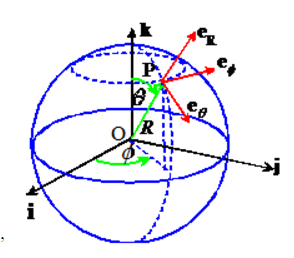
\includegraphics{octree/ex_images/oct_ex_tran.png}}
    \caption{Coordinate transformation}
    \label{octree_fig:oct_ex_hollow_sphere_tran}
  \end{figure}
  
\paragraph{}
In the example, $a = 10,b = 50, E=20,\nu = 0.2,P_a = 10$. For simplification, only a quarter of the sphere is analysed as shown in fig.~\ref{oct_fig:ex_hollow_sphere_meshP}

\begin{figure}[h!]
  \centering
  \scalebox{0.5}{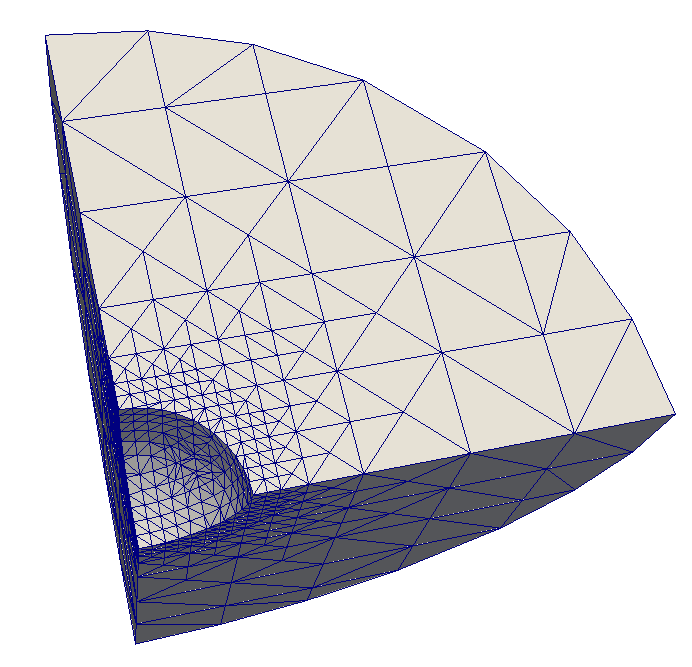
\includegraphics{octree/ex_images/oct_ex_mesh.png}}
  \caption{Mesh of the problem}
  \label{oct_fig:ex_hollow_sphere_meshP}
\end{figure}

Stress boundary in Eq.~\ref{oct_eq:ex_sphere_hole_bond_str} condition is applied on two spherical surfaces.
\begin{subequations}
    \begin{align}
    \sigma_{RR}(R=a,\phi,\theta) & = \frac{p_aa^3-p_bb^3}{b^3-a^3} - \frac{(p_a-p_b)b^3a^3}{(b^3-a^3)R^3}\\
    u_z(x,y,0) &= 0\\
    u_y(x,0,z) & = 0 \\
    u_x(0,y,z) & = 0
  \end{align}
\label{oct_eq:ex_sphere_hole_bond_str}
\end{subequations}

The convergence study is plotted in Fig.~\ref{oct_fig:ex_hollow_sphere_conv}
\begin{figure}[h!]
    \centering
    \scalebox{0.5}{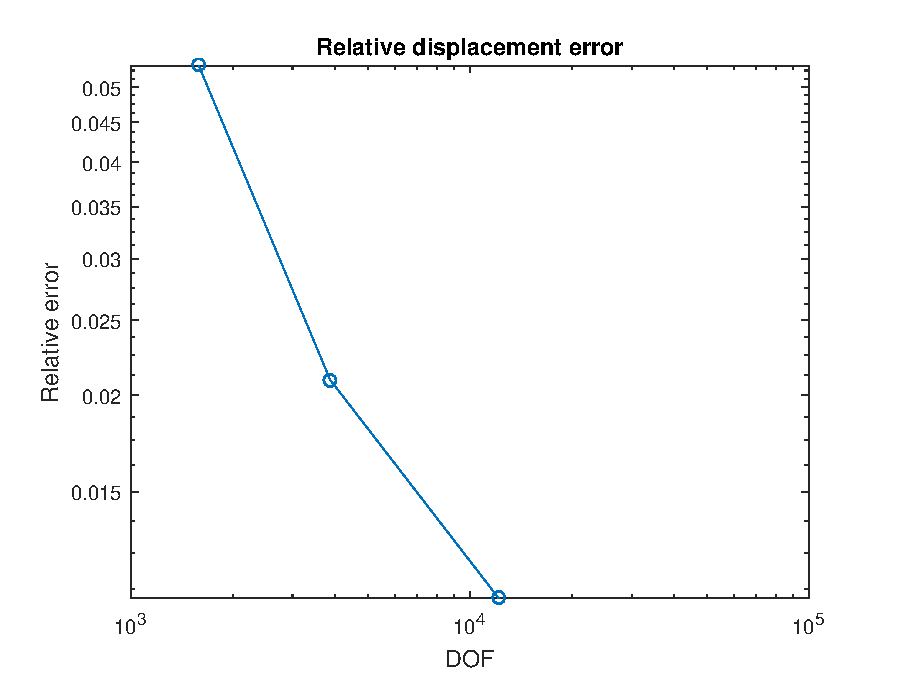
\includegraphics{octree/ex_images/ex_sphere_hole_conv.eps}}
    \caption{Convergence of displacement error}
    \label{oct_fig:ex_hollow_sphere_conv}
  \end{figure}
\subsection{Capsule Cutting From the Cuboid with Bending}
\paragraph{}
The example is a capsule section cutting from a cuboid with pure bending illustrated in Fig.~\ref{oct_fig:ex_caplus_layout} and the generated mesh is plotted in Fig.~\ref{oct_fig:ex_caplus_mesh1.png}.
\begin{figure}[h!]
  \centering
  \scalebox{.5}{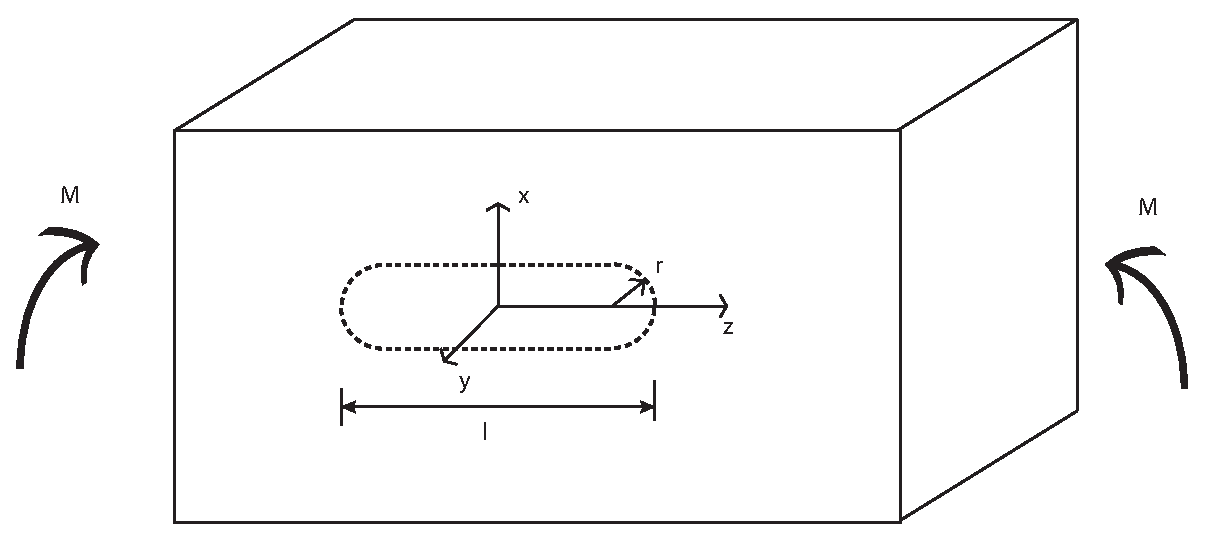
\includegraphics{octree/ex_images/oct_ex_caplus_rect.eps}}
  \caption{Problem layout}
  \label{oct_fig:ex_caplus_layout}
\end{figure}
%
\begin{figure}[h!]
  \centering
  \scalebox{.3}{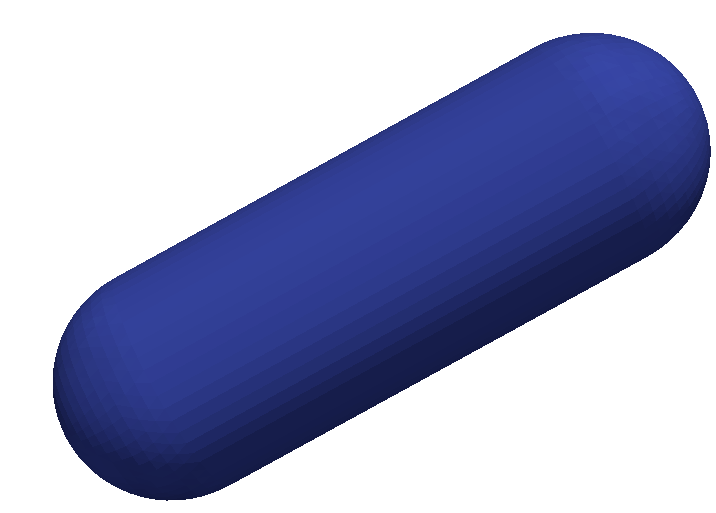
\includegraphics{octree/ex_images/oct_ex_caplus_geo.png}}
  \caption{Geometry of the capsule}
  \label{oct_fig:ex_caplus_geo}
\end{figure}
%
\begin{figure}[h!]
    \centering
    \begin{subfigure}[b]{1\linewidth}
        \centering
        \scalebox{.3}{
            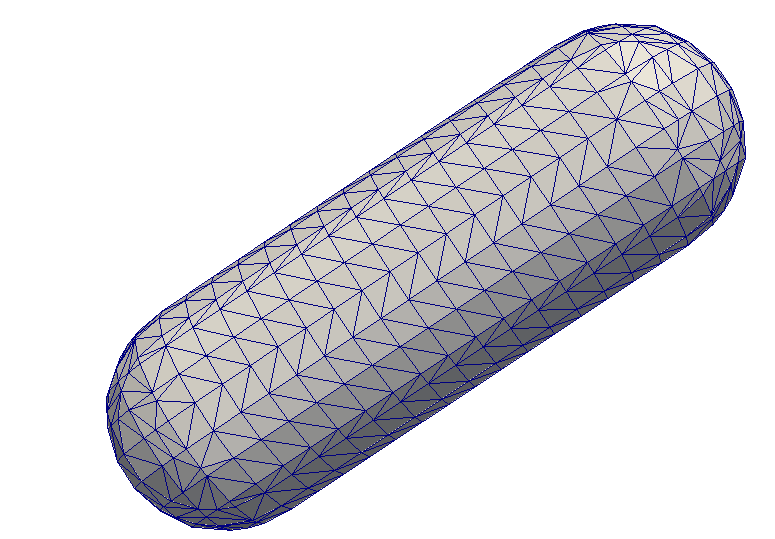
\includegraphics{octree/ex_images/oct_ex_caplus_mesh1.png}
        }
    \end{subfigure}
    \begin{subfigure}[b]{1\linewidth}
        \centering
        \scalebox{.3}{
            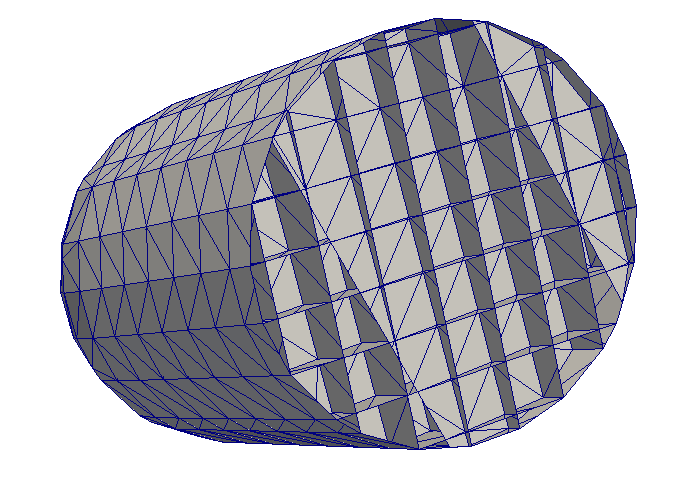
\includegraphics{octree/ex_images/oct_ex_caplus_mesh2.png}
        }
    \end{subfigure}
    \caption{Mesh of the Capsule}
    \label{oct_fig:ex_caplus_mesh1.png}
\end{figure}
%
The displacement analytical solution \citep{Tim1951} is applied on the outer surface of the capsule as the boundary condition and the displacement and \hl{the} stress (Eq.~\ref{eqn:caplus_stress}) inside is compared to the analytical solution.
All stress component \hl{except} $\sigma_z$ is zero.

\begin{subequations}
\begin{align}
  u_x &= -\frac{1}{2R}\left[z^2 + \nu \left(x^2 - y^2 \right)\right]\\
  u_y &= -\frac{\nu xy}{R}\\
  u_z &= \frac{xz}{R} 
  \label{eqn:capluse_displacement}
\end{align}
\end{subequations}

\begin{equation}
  \sigma_x = \frac{Ex}{R}
  \label{eqn:caplus_stress}
\end{equation}
%
In the numerical calculation, The dimension of the outer cuboid will not affect the result because of the independence of the analytical solution (Eq.\ref{eqn:capluse_displacement}).
6-nodes triangular element\hl{s are} used to achieve an exact solution.
The geometric properties are: $l=\SI{100}{\meter}$ and $r=\SI{17.5}{\meter}$
The material properties are: $\nu=0.2$ and $E=\SI{30}{\newton \per \square \meter}$.
The error of the displacement is calculated as followed.
\begin{subequations}
\begin{align}
e_u &= \frac{||u_{ex} - u||}{||u_{ex}||}\\
e_s &= \frac{||\sigma_{ex} - \sigma||}{||\sigma_{ex}||}
\end{align}
\end{subequations}
%
The error of the displacement norm is $1.7563\times 10^{-14}$ and the error of the stress norm is $1.3184\times 10^{-9}$.

\subsection{Wall lamp}
\paragraph{}
In this example, a wall lamp illustrated in Fig.~\ref{oct_ex:lamp_geo_bc} with gravity only is considered.
The material properties are:  Young’s modulus $E = \SI{20}{\newton \per \square \meter}$, Poisson’s ratio $\nu = 0.3$ and density $\rho = \SI{2}{\kilo \gram \per \cubic \meter}$.
\begin{figure}
    \centering
    \scalebox{0.5}{
        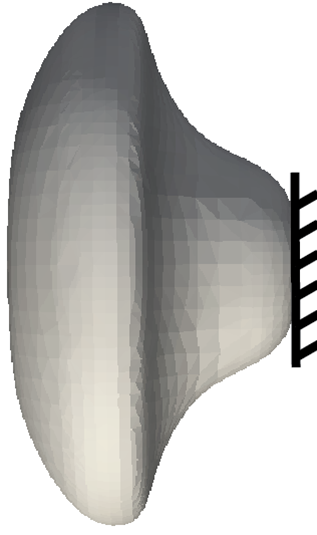
\includegraphics{octree/ex_images/lamp_geo_bc.png}
    }
    \caption[Boundary condition of the wall lamp]{Boundary condition of the wall lamp}
    \label{oct_ex:lamp_geo_bc}
\end{figure}

\paragraph{}
The geometric model is extracted from the AutoCAD as illustrated in Fig.~\ref{oct_ex:lamp_cad}.
\begin{figure}[!ht]
    \centering
    \scalebox{0.5}{
        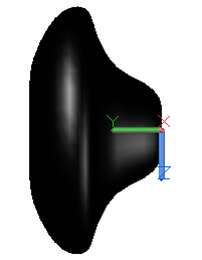
\includegraphics{octree/ex_images/lamp_cad.png}
    }
    \caption[CAD drawing of the wall lamp]{CAD drawing of the wall lamp}
    \label{oct_ex:lamp_cad}
\end{figure}
%
The background mesh before cutting is shown in Fig.~\ref{oct_ex:lamp_mesh_bg}.
\begin{figure}[!ht]
    \centering
    \begin{subfigure}[b]{0.49\linewidth}
        \centering
        \scalebox{0.65}{
            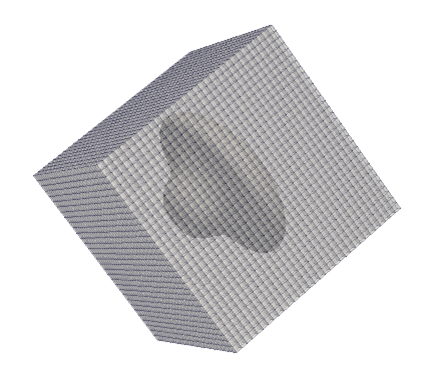
\includegraphics{octree/ex_images/lamp_mesh_bg.png}
        }
    \end{subfigure}
    \begin{subfigure}[b]{0.49\linewidth}
        \centering
        \scalebox{0.65}{
            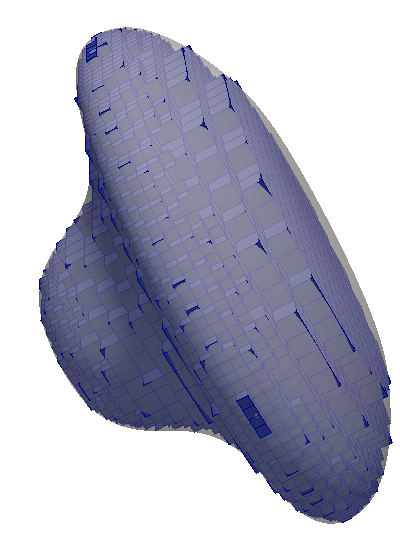
\includegraphics{octree/ex_images/lamp_mesh_bg_2.png}
        }
    \end{subfigure}
    \caption[Background mesh of the wall lamp]{Background mesh of the wall lamp; left: background mesh; right: background mesh around the boundary}.
    \label{oct_ex:lamp_mesh_bg}
\end{figure}
%
The generated mesh are plotted in Fig.~\ref{oct_ex:lamp_mesh}.
\begin{figure}[!ht]
    \centering
    \begin{subfigure}[b]{1\linewidth}
        \centering
        \scalebox{0.75}{
            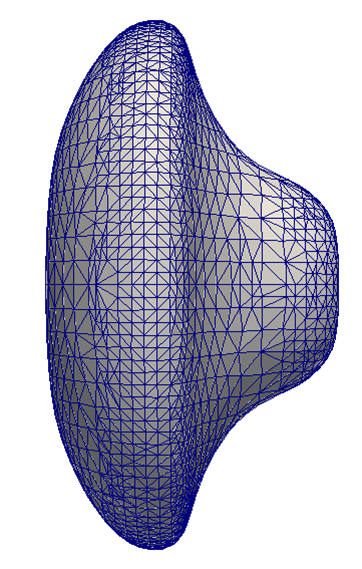
\includegraphics{octree/ex_images/lamp_mesh.png}
        }
    \end{subfigure} \\
    \begin{subfigure}[b]{0.48\linewidth}
        \centering
        \scalebox{0.75}{
            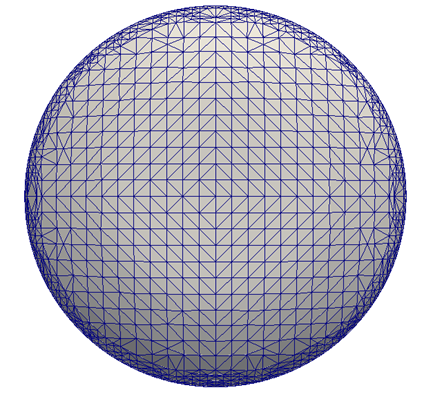
\includegraphics{octree/ex_images/lamp_mesh_front.png}
        }
    \end{subfigure}
    \begin{subfigure}[b]{0.48\linewidth}
        \centering
        \scalebox{0.75}{
            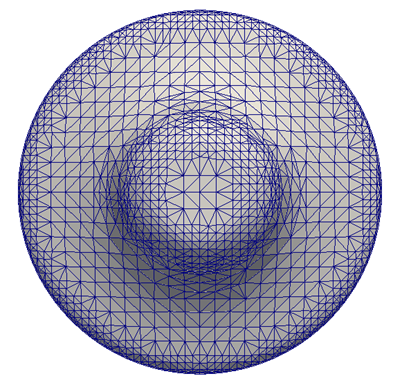
\includegraphics{octree/ex_images/lamp_mesh_back.png}
        }
    \end{subfigure}
    \caption[Mesh of the wall lamp]{Mesh of the wall lamp}
    \label{oct_ex:lamp_mesh}
\end{figure}
%
The displacement is plotted as the deformed shape in Fig.~\ref{oct_ex:lamp_deformed_shape}.
\begin{figure}[!ht]
    \centering
    \scalebox{0.5}{
        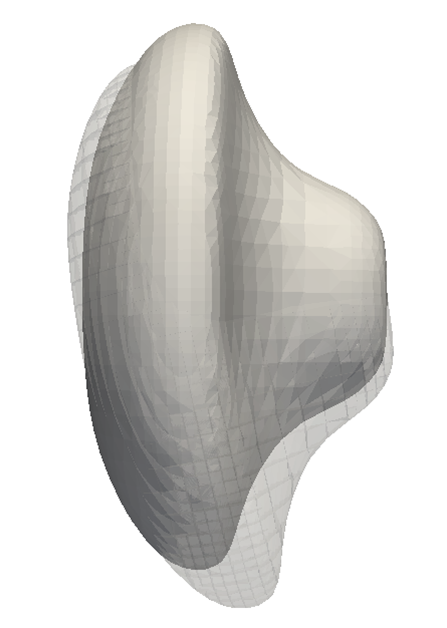
\includegraphics{octree/ex_images/lamp_deformed_shape.png}
    }
    \caption[Deformed shape of the wall lamp]{Deformed shape of the wall lamp}
    \label{oct_ex:lamp_deformed_shape}
\end{figure}

\subsection{Meshing examples}
\paragraph{}
In this section, some other mesh examples with irregular geometric boundaries are considered.
% Fig.~\ref{} and Fig.~\ref{qdt_ex:mesh_wolli_logo} show the mesh generated for a flower input.
% Fig.~\ref{} and Fig.~\ref{qdt_ex:mesh_wolli_logo_sharp} highlight the sharp corner treatment of the algorithm.

\begin{figure}
    \centering
    \scalebox{0.25}{
        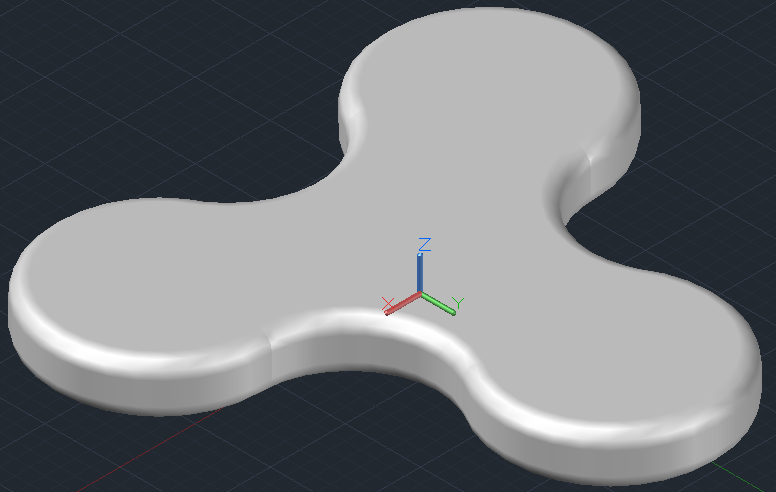
\includegraphics{octree/ex_images/spinner_cad.png}
    }
    \caption[CAD design for spinner]{CAD design for spinner}
    \label{oct_ex:mesh_spinner_cad}
\end{figure}

\begin{figure}
    \centering
    \begin{subfigure}[b]{0.49\linewidth}
        \centering
        \scalebox{0.25}{
            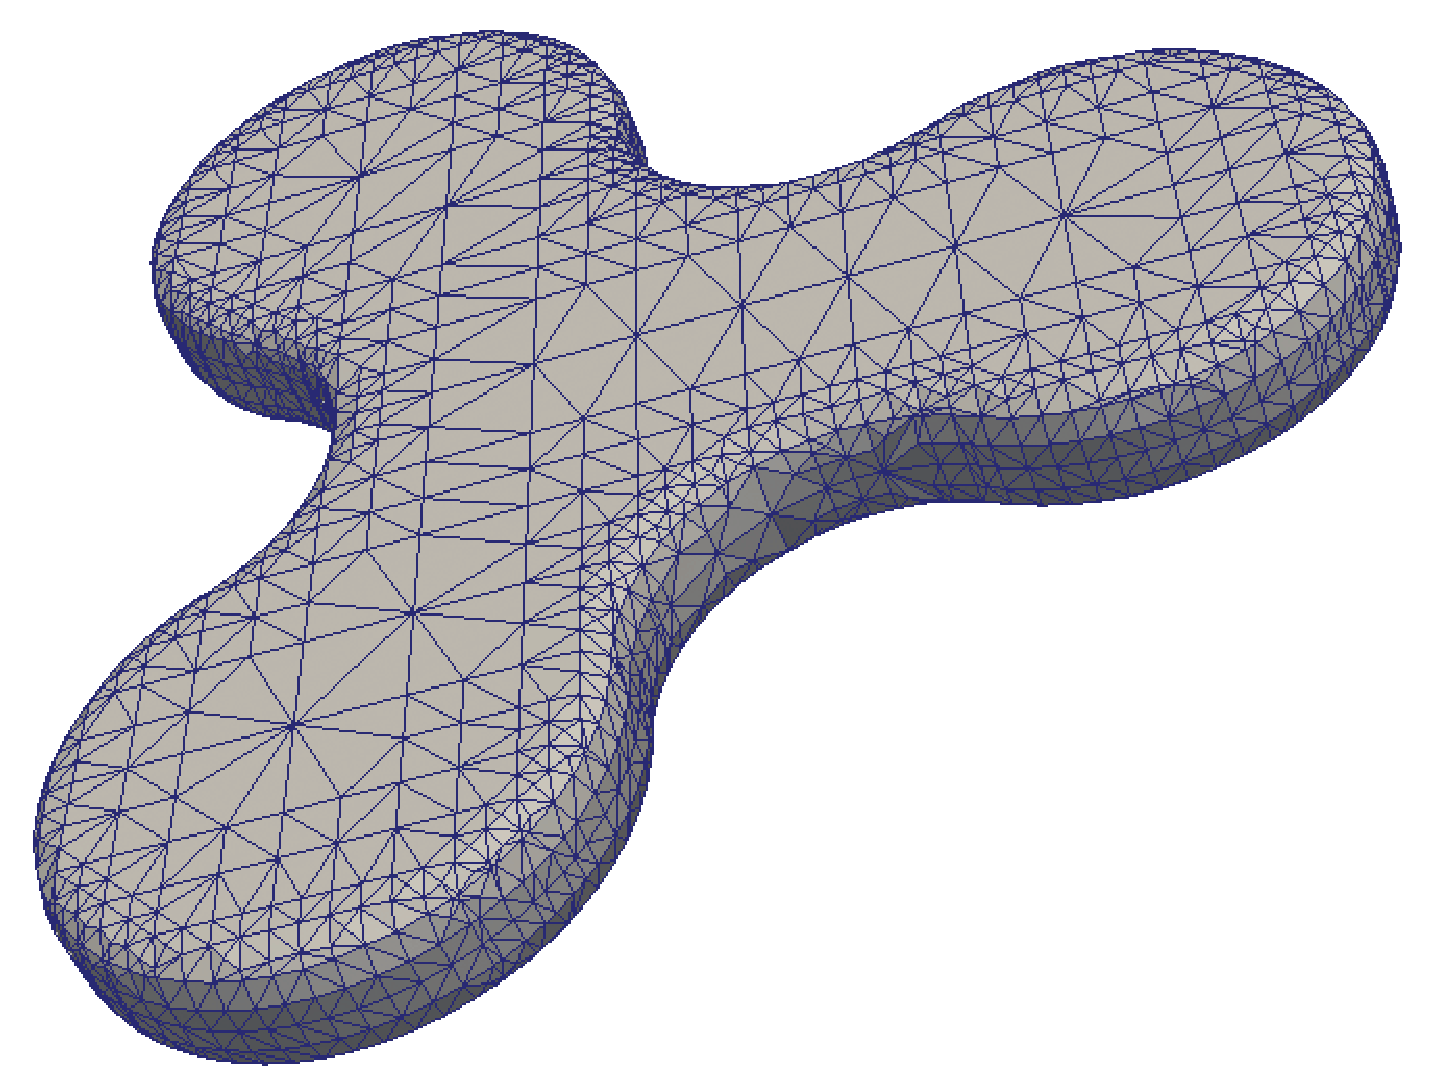
\includegraphics{octree/ex_images/spinner_full.eps}
        }
    \end{subfigure}
    \begin{subfigure}[b]{0.49\linewidth}
        \centering
        \scalebox{0.25}{
            \includegraphics{octree/ex_images/spinner_top.eps}
        }
    \end{subfigure} \\
    \begin{subfigure}[b]{0.49\linewidth}
        \centering
        \scalebox{0.25}{
            \includegraphics{octree/ex_images/spinner_side.eps}
        }
    \end{subfigure}
    \begin{subfigure}[b]{0.49\linewidth}
        \centering
        \scalebox{0.25}{
            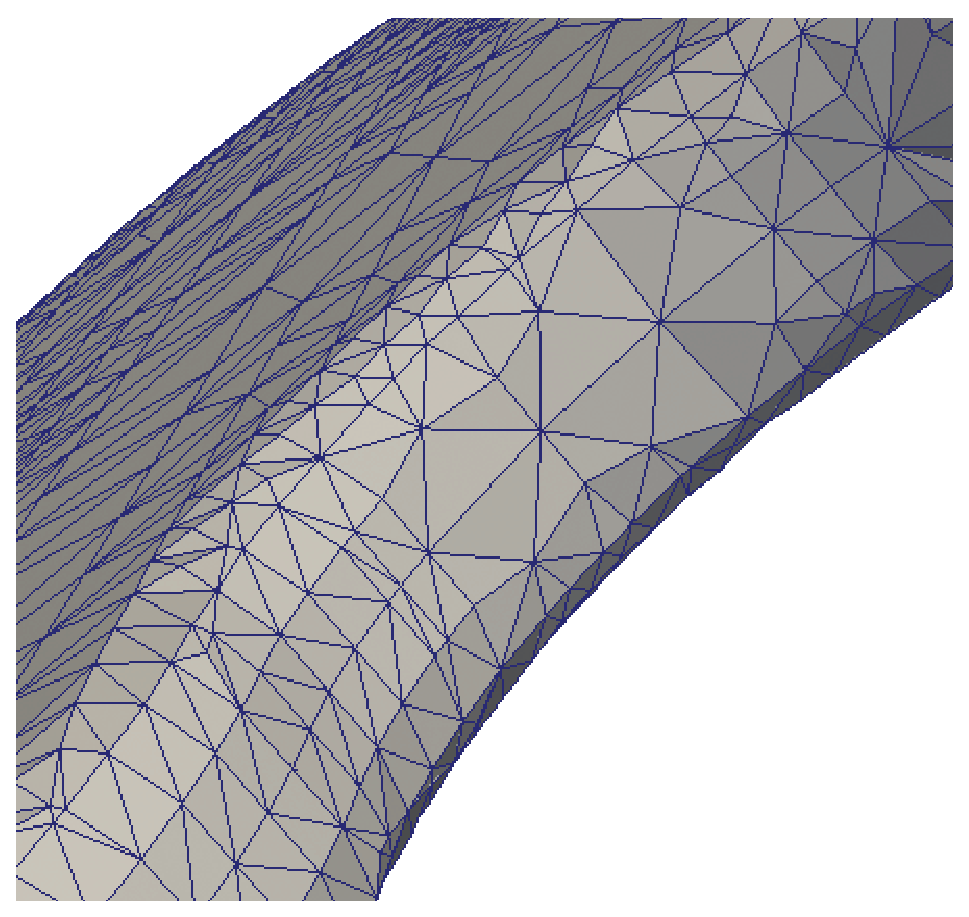
\includegraphics{octree/ex_images/spinner_part.eps}
        }
    \end{subfigure}
\end{figure}

\section{Conclusions}
\paragraph{}
In this chapter, a projection is conducted after the octree mesh is generated from the STL file.
Geometric exact is retained by projecting intersections on the triangular surfaces back to original NURBS surfaces or by replacing the intersection calculation with finding that between the edge of the element and the NURBS surface directly. 
Both of the projecting and the intersection calculating are accelerated by utilizing the strong convex hull property of the NURBS.
The proposed method is able to generate the mesh from an arbitrary geometric input and shows higher accuracy compared to conventional method.